\chapter{Überblick über Modern OpenGL}
\label{cha:modern-opengl}

\section{Von Fixed Pipeline zu Shadern}
Mit der Abkehr von der Fixed Pipeline begann die Ära von Modern OpenGL. Seit dem ist es möglich mit eigenen Shader-Programmen, meist geschrieben in GLSL, die einzelnen Stufen der Renderpipline anzupassen. Anfangs beschränkten sich die Stufen auf den Vertex Shader und den Fragment Shader. Im Laufe der Zeit sind noch eine Vielzahl von weiteren programmierbaren Shader-Stufen hinzu gekommen.

Die Abkehr von der Fixed Pipeline erlaubte völlig neue Konzepte im Echtzeit-Rendering. Anfangen von eigenen, anstatt fest vorgegeben, Beleuchtungsmodellen (siehe \fref{chap:pbr}) hin zu komplett Fragment Shader basierten Grafikdemos\footnote{https://www.shadertoy.com/view/Xtf3Rn} und gänzlich neuen Echzeit-Rendering Konzepten\footnote{http://iquilezles.org/www/articles/raymarchingdf/raymarchingdf.htm}.

Während ursprünglich der Szene-Graph fest von OpenGL vorgegeben war und Vertices mindestens einmal jeweils und \textit{einzeln} von der CPU auf die GPU geladen werden mussten, änderte sich auch dies fundamental. Mit dem Ende der Fixed Pipeline wurden auch Buffer-Objekte immer wichtiger, so dass ganze Speicherbereiche direkt befüllen oder manipuliert werden konnten. Der Overhead Vertices zur Grafikkarte zu schicken reduzierte sich entsprechend deutlich. Inzwischen gibt es eine Vielzahl von unterschiedlichen Buffer-Typen für unterschiedliche Zwecke, bis hin zu generischen Buffern, die auschließlich von Compute Shadern befüllt werden können, ohne dass deren Daten jemals von der CPU über den Bus geschickt werden mussten.

Schließlich konnte der bis dato wesentliche Flaschenhals und limitierende Faktor, der Bus zur Grafikkarte, optimal genutzt werden, und war oft nur noch in initialen oder sporadischen Befüllungsvorgängen limitierend. Wie so oft tat sich entsprechend ein neuer Engpass auf. Dieser lag nun, und liegt oft noch immer, in der Implementierung der API, dem Treiber.

\section{Treiber Overhead}

Dabei ist die OpenGL API und ihre Treiberimplementierung nicht per se ein Flaschenhals, doch erlaubt die gewachsene und rückwärtskompatibel gehaltene API unterschiedliche Pfade zum annähernd gleichen Ziel. Einige ältere Pfade bringen oft mehr Overhead mit sich, neuere erlauben die effektive Reduzierung der API Aufrufe. \ac{AZDO}, eine Initiative von AMD, nVidia und Intel, versucht seit ein bis zwei Jahren die schnelleren Pfade bei den Entwicklern bekannter zu machen. Zu den sc\ac{MDI}, zu nutzen.

\paragraph{\acl{MDI}} 
\ac{MDI} beschreibt das Ausführen von mehreren Draw-Calls mit einen API Aufruf. Zuvor werden die für die Aufrufe notwendigen Parameter in OpenGL Buffer geschrieben. Die Parameter können entweder von der CPU aus bestimmt werden oder direkt von der GPU (z.B. durch View-Frustum Culling auf der GPU).

\begin{figure}
	\label{fig:opengl-pfade}
	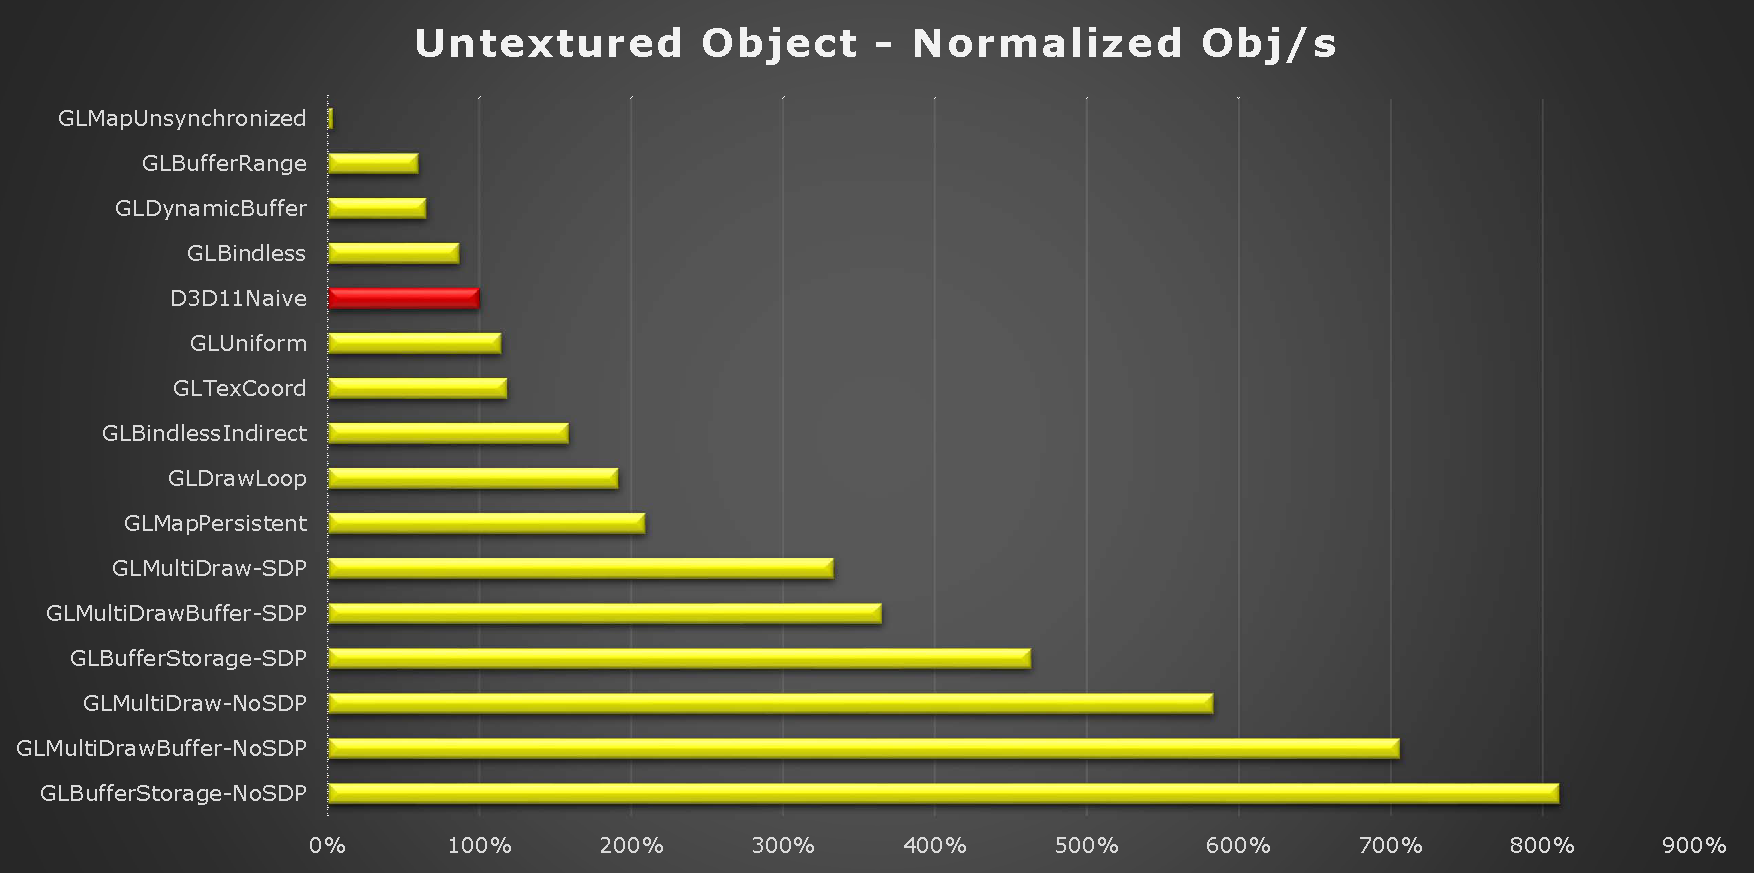
\includegraphics[width=\textwidth]{img/opengl-spread}
	\caption{Unterschiede in den Pfaden \parencite[Seite 98]{Everitt2014}}
\end{figure}


Große Buffer (z.B. für Shader), Daten in Blöcken anstatt einzeln


\ac{DSA}

\cite{gamedevnet:glnext}
